   
\documentclass[11pt]{article}
\usepackage{amsmath,amsthm,verbatim,amssymb,amsfonts,amscd, graphicx}
\usepackage{graphicx}
\usepackage{listings}
\usepackage{float}
\usepackage{inconsolata}
\usepackage{url}
\usepackage{titlesec}
\setcounter{secnumdepth}{4}




\graphicspath{{./times/}}
\topmargin0.0cm
\headheight0.0cm
\headsep0.0cm
\oddsidemargin0.0cm
\textheight23.5cm
\textwidth16.5cm
\footskip1.0cm

\titleformat{\paragraph}
{\normalfont\normalsize\bfseries}{\theparagraph}{1em}{}
\titlespacing*{\paragraph}
{0pt}{3.25ex plus 1ex minus .2ex}{1.5ex plus .2ex}


\begin{document}
\title{CS 5220\\ Project 3 - Floyd-Warshall Algorithm}
\author{Eric Gao (emg222)\\ Elliot Cartee (evc34)\\ Sheroze Sheriffdeen(mss385)}
\maketitle

\section{Introduction}
The Floyd-Warshall algorithm computes the pair-wise shortest path lengths given a graph with a metric. The computational pattern of this algorithm is very much akin to matrix multiplication. If $l_{ij}^s$ represents the the length of the shortest path from node $i$ to $j$ in at most $2^s$ steps, \cite{writeup} then
\begin{equation}
	l_{ij}^{s+1} = \min_k \{ l_{ik}^s + l_{kj}^s \}
\end{equation} 

\section{Design Decisions}
 
\subsection{Parallel Tuning}

Since the Floyd-Warshall algorithm is structured very similarly to matrix multiplication, we decided to try taking some of the tuning methods used in the first project on matrix multiplication, and applying them to the Floyd-Warshall algorithm.

The first of these methods is using a blocking scheme, so that updating the shortest path lengths is done through repeated calls to a small kernel. Since the size of this small kernel is known at compile-time, the compiler is able to optimize this small kernel extremely efficiently. Currently our implementation of blocking only works when the number of vertices is divisible by the block size, but we plan to correct this soon.

The second method was to change the loop ordering, so that in the innermost loop, memory is being accessed with unit stride, which increases performance.

As the project goes on, we also hope to add other optimizations attempted in the matrix multiplication project, such as copying the blocks into a contiguous chunk of memory.

\subsection{Message Passing Interface}

In addition to the tuned parallel implementations, we explored an approach that uses the Message Passing Interface to achieve parallelism. In the MPI implementation, each process handles a certain region of the graph. To prevent a master process orchestrating the distance computation, we ideally want each process to only wait for information from the relevant part of the graph. To that end, we take the adjacency matrix on which the Floyd-Warshall algorithm is run and partition the graph by chunks of columns. Then each processors is responsible for update a contiguous sequence of columns in the matrix.

\begin{figure}[H]
\centering
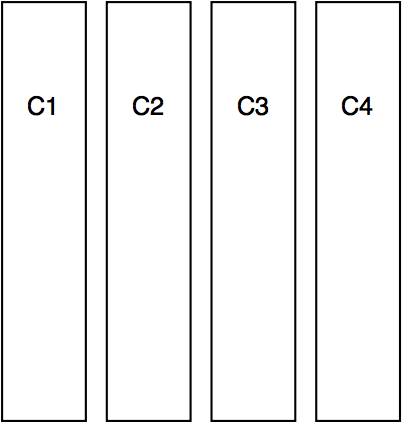
\includegraphics[scale=0.25]{initial_partition.png}
\caption{Initial partition of the graph where each $C_i$ is a sequence of columns}
\label{fig:init_part}
\end{figure}

Now each sequence of columns owned by a processor can be decomposed into square blocks. To compute the next iteration of the Floyd-Warshall algorithm for a single block, say block number $i$ in processor $2$, we need the $i^{th}$ block from all other processors.

\begin{figure}[H]
\centering
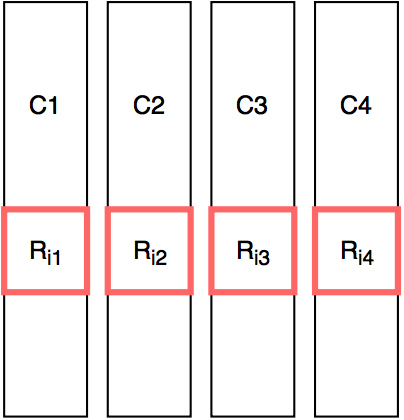
\includegraphics[scale=0.25]{allgather.png}
\caption{For block $R_{i1}$ we need the $i^{th}$ block from all other processors}
\label{fig:allgather}
\end{figure}

Therefore, we do an \texttt{MPI\_Allgather} operation which gathers the $i^{th}$ block from all the processors and recreates the $i^{th}$ row chunk in all processors. Now, we can update block $R_{ij}$ for all $j$ processors. 

\begin{figure}[H]
\centering
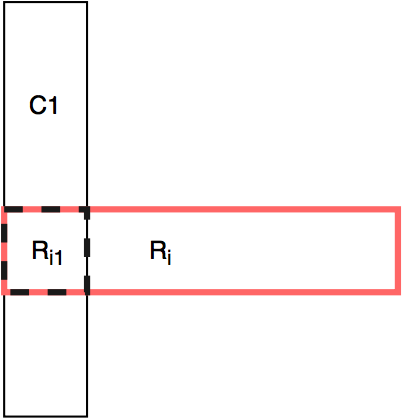
\includegraphics[scale=0.25]{row_col.png}
\caption{Updating the $i^{th}$ square block by processor 1 using row chunk $i$}
\label{fig:row_col}
\end{figure}

The \texttt{MPI\_Allgather} is then repeated until all square blocks have completed a step in the Floyd-Warshall algorithm. Each processor individually checks whether an update was made to their sequence of columns. To complete the iteration, we perform a \texttt{MPI\_Allreduce} operation to check whether any update was made across all processors. If an update was made, we continue the iteration. Otherwise, all processors terminate and the solution is reached.

\subsubsection{Advantages}

The MPI approach improves upon a serial implementation of the algorithm due to its ability to compute updates to multiple regions of the graph in parallel.
 
The MPI approach makes each processor be responsible of a contiguous sequence of columns in the graph. To update a a square block in this sequence of columns, the processor needs to recreate only the corresponding sequence of rows. Therefore, if the width of the sequence of columns is $d$ and the side length of the graph is $n$, each processor only needs to hold $2nd$ information in memory instead of $n^2$. On larger graphs, this decrease in memory footprint will prevent thrashing since the space scales as $O(n)$ instead of $O(n^2)$ and will show improvements in performance over the OpenMP version.

\subsubsection{Disadvantages}
On smaller graphs, the communication and synchronization overhead  of MPI may cause a decrease in performance.

\subsubsection{Implementation}
The MPI implementation can be found in \texttt{path-mpi.c}. We are still in the process of ironing out bugs in the implementation and hope to have a complete solution by the final report. Furthermore, if time permits, we aim to explore the Cannon's algorithm to improve upon the current MPI scheme. \cite{cannon}

\section{Analysis}

\subsection{Original Implementation}
\subsubsection{Profiling} \label{sec:prof_orig}

Profiling the original solution shows that the most CPU time goes into the square function and significant portion of that time is considered by VTune to be ideal. The next most expensive functions in terms of CPU time is the barrier and the reduction in OpenMP due to the high spin times. 

\lstinputlisting[basicstyle=\tiny\ttfamily]{./profiling/path_original.txt}

\subsubsection{Scaling Study} \label{sec:speedup_orig}

The speedup plots of the original solution shows linear improvement in performance but an exponential decrease in efficiency as shown in figure~\ref{fig:ws_orig}. This can be attributed to the increased overhead in synchronization and spin time.

\begin{figure}[H]
\centering
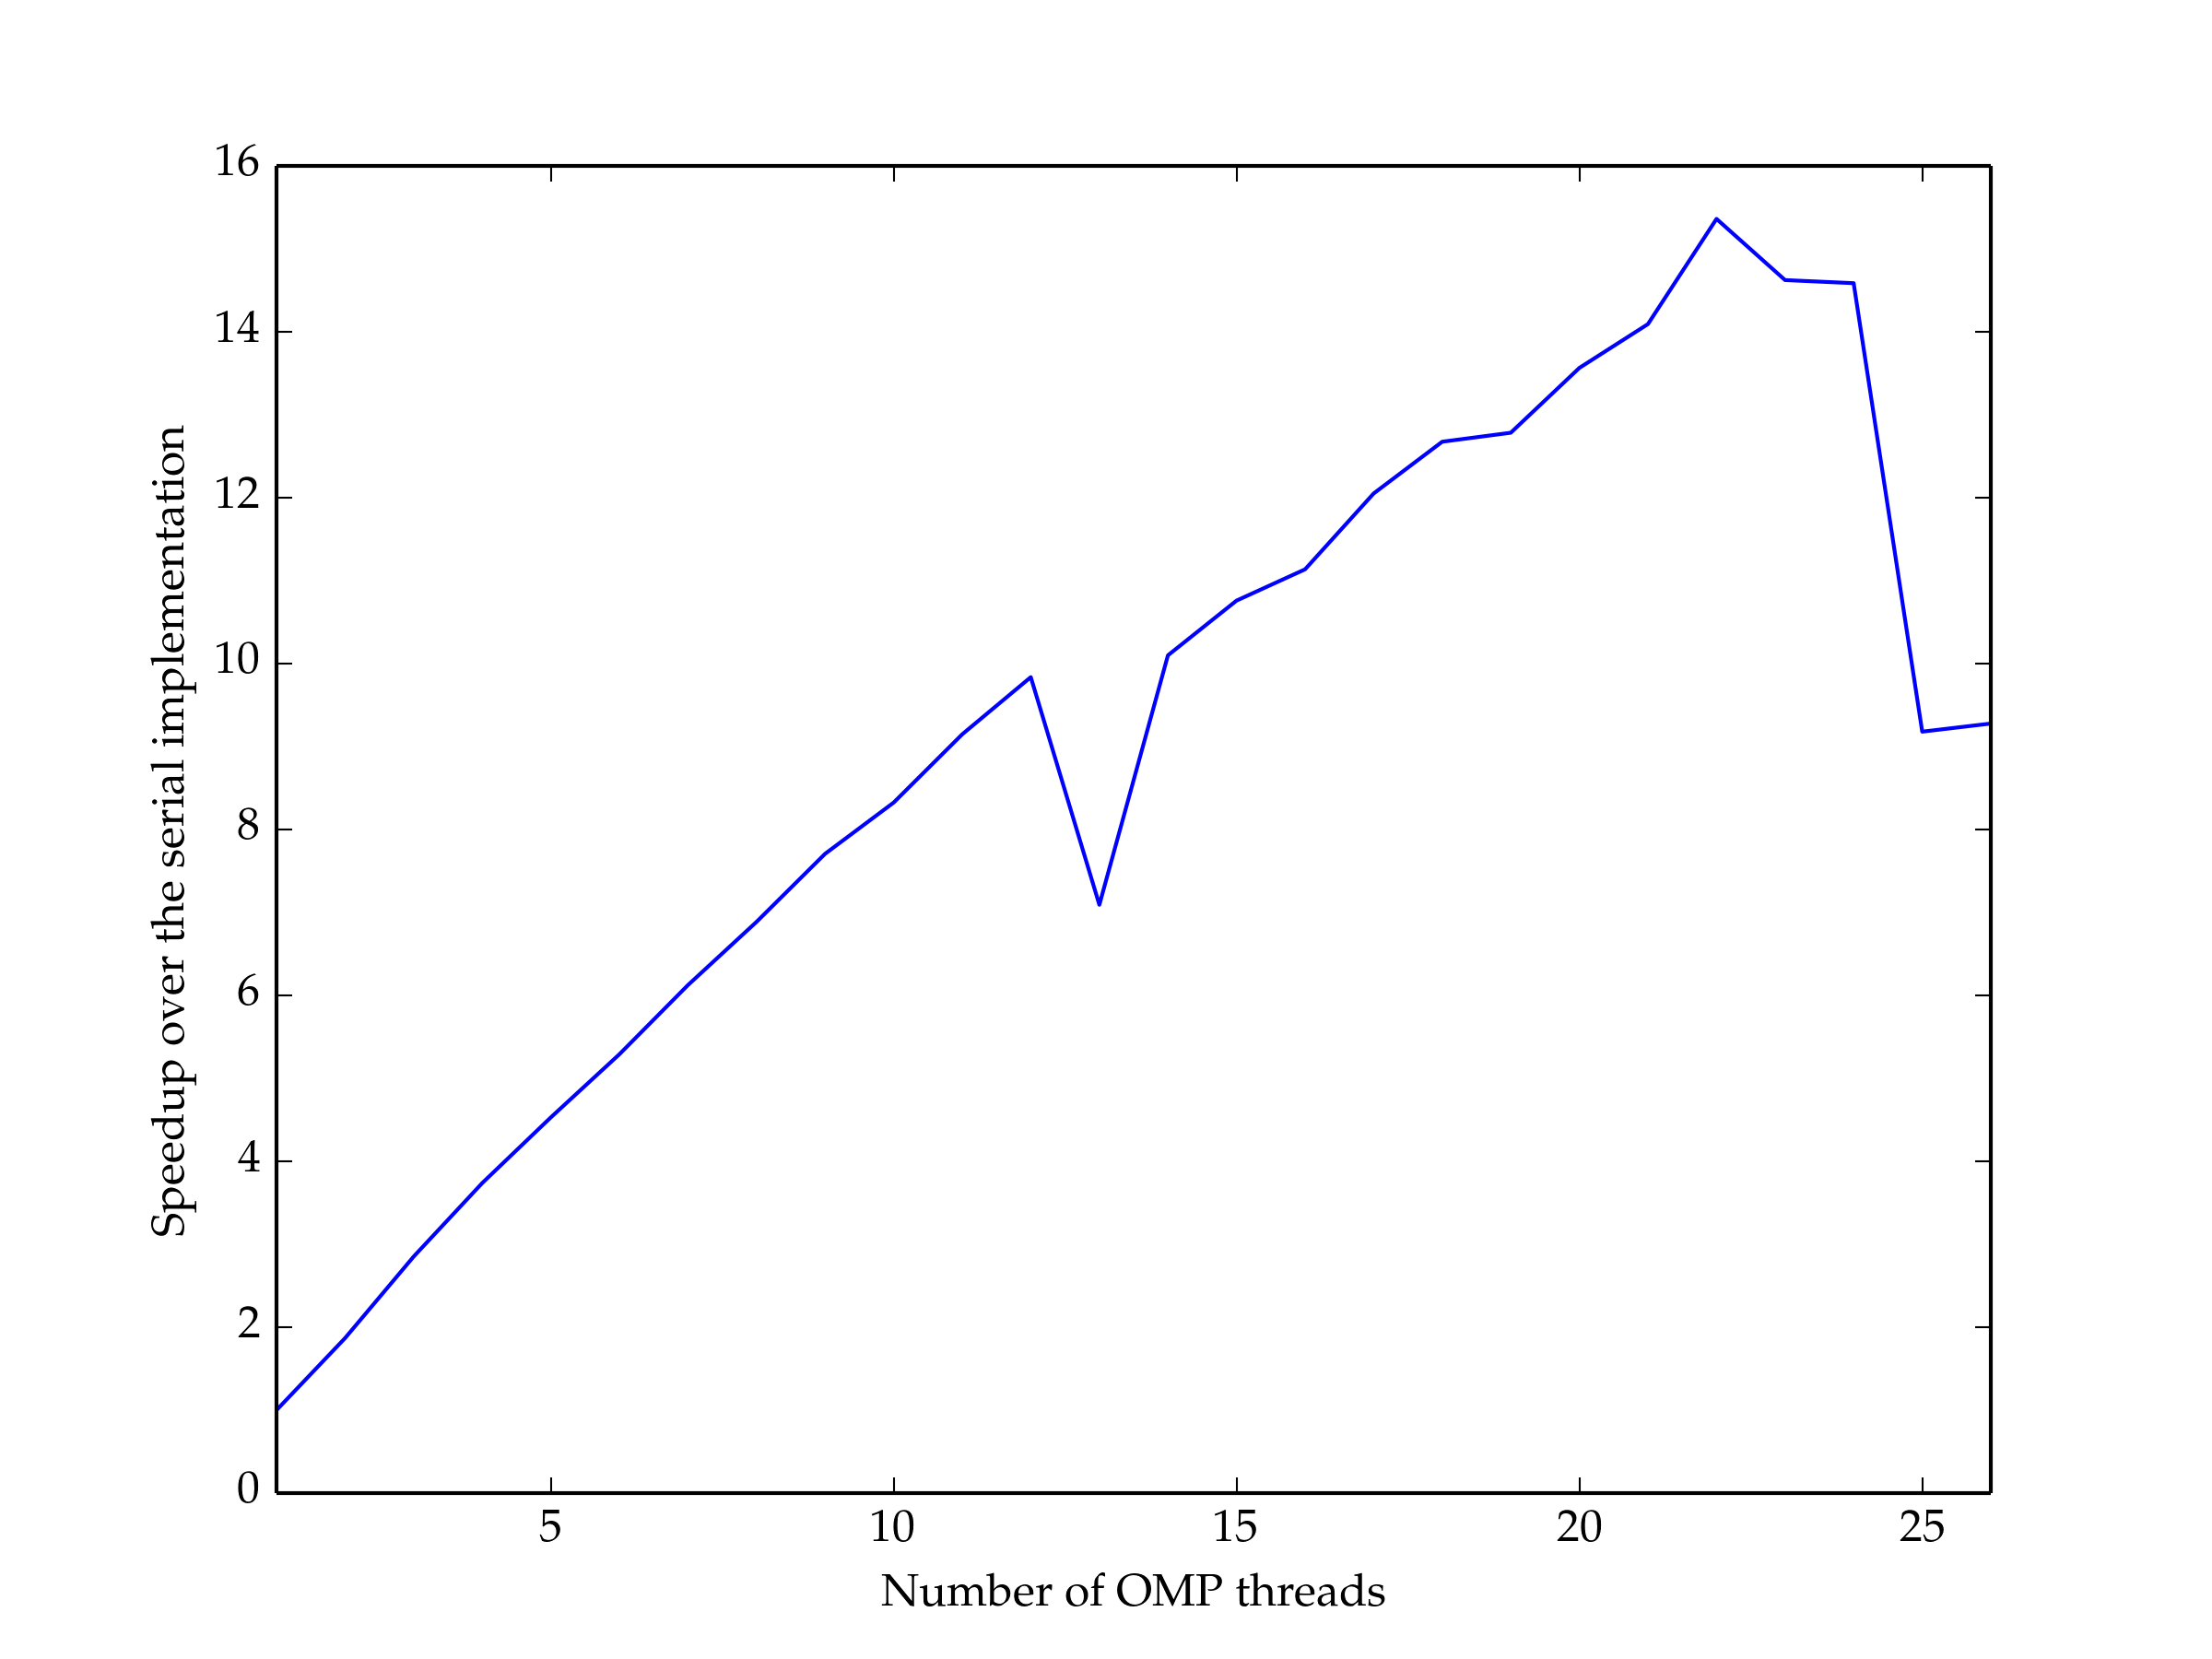
\includegraphics[scale=0.5]{./scaling_studies/strong_scaling_original.png}
\caption{Strong scaling study of the original solution}
\label{fig:ss_orig}
\end{figure}

\begin{figure}[H]
\centering
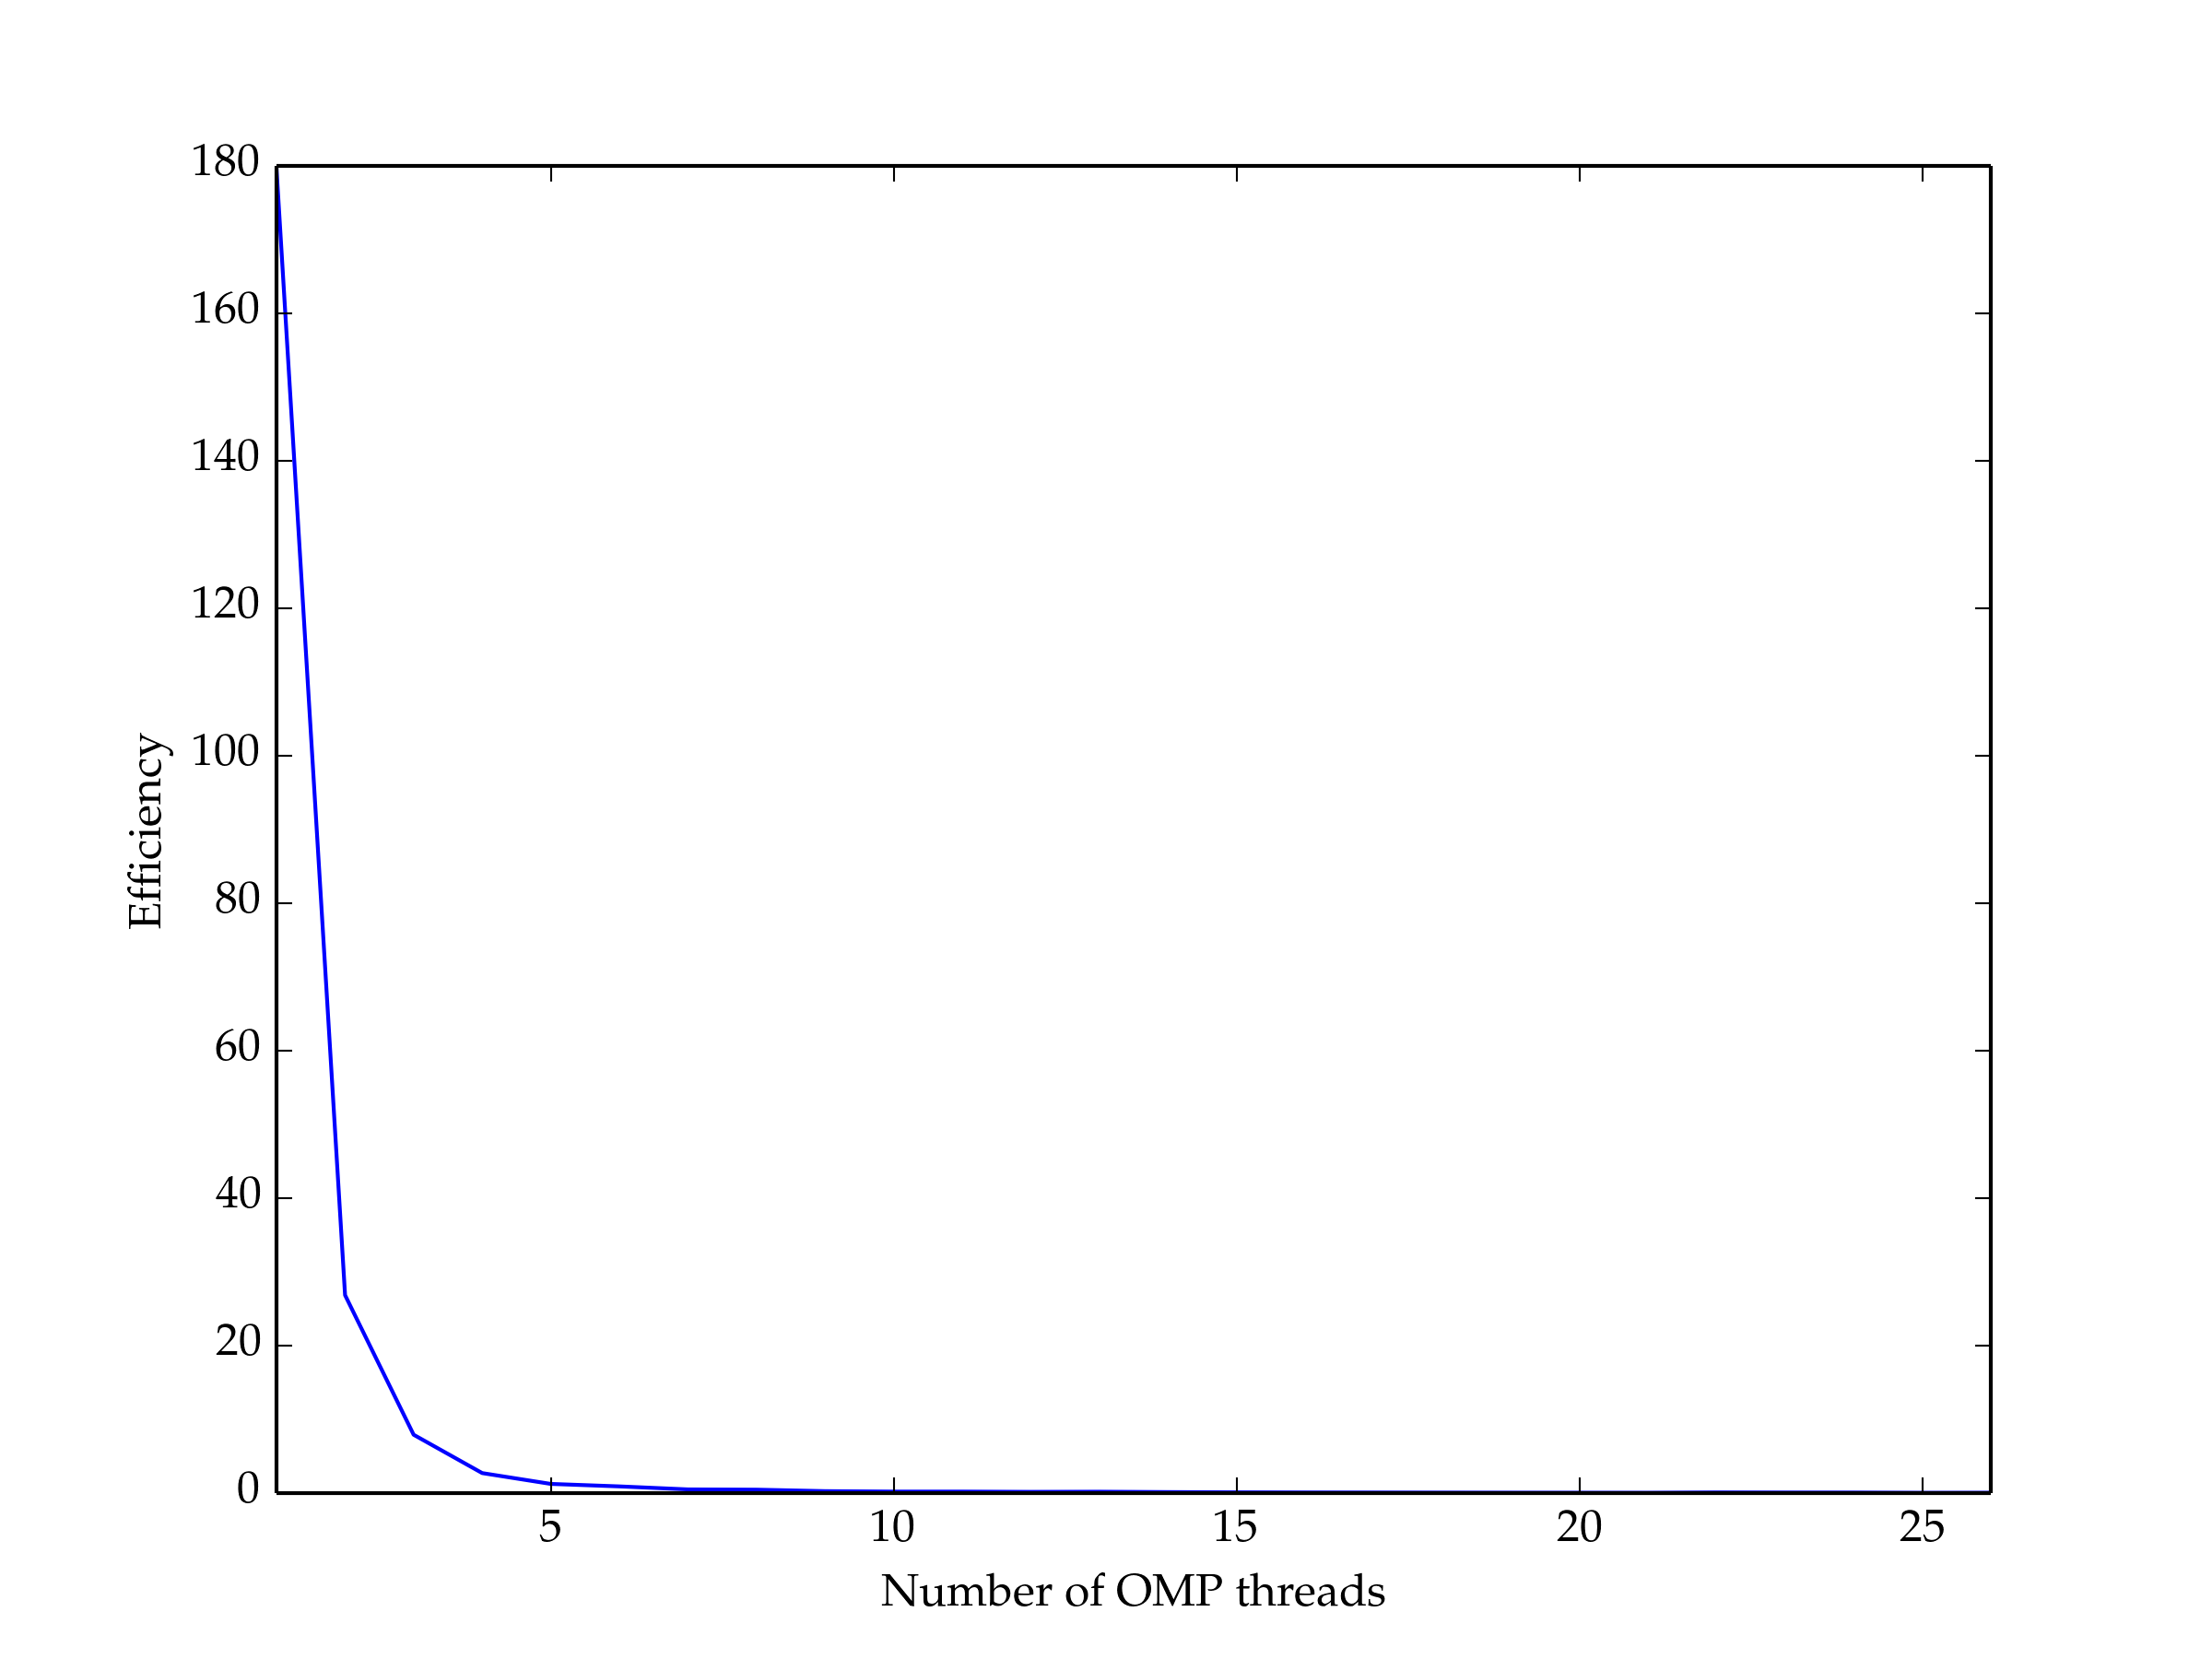
\includegraphics[scale=0.5]{./scaling_studies/weak_scaling_original.png}
\caption{Weak scaling study of the original solution}
\label{fig:ws_orig}
\end{figure}

The strong scaling study was performed on a graph with 2000 nodes. The weak scaling varies the number of threads but keeps the problem size per processor be 1000 nodes. 

\subsection{Tuned Parallel Implementation}

\subsubsection{Profiling} \label{sec:prof}

Unfortunately, we ran into some technical difficulties with VTune Amplifier XE, and were unable to profile our tuned OpenMP implementation in time for this intermediate report.

\subsubsection{Scaling Study} \label{sec:speedup}

Although the scaling studies for the tuned parallel implementation times show similar speedup and efficiency patterns as the original solution, the overall time taken to achieve the solution is lower than the original OpenMP solution. 
\begin{figure}[H]
\centering
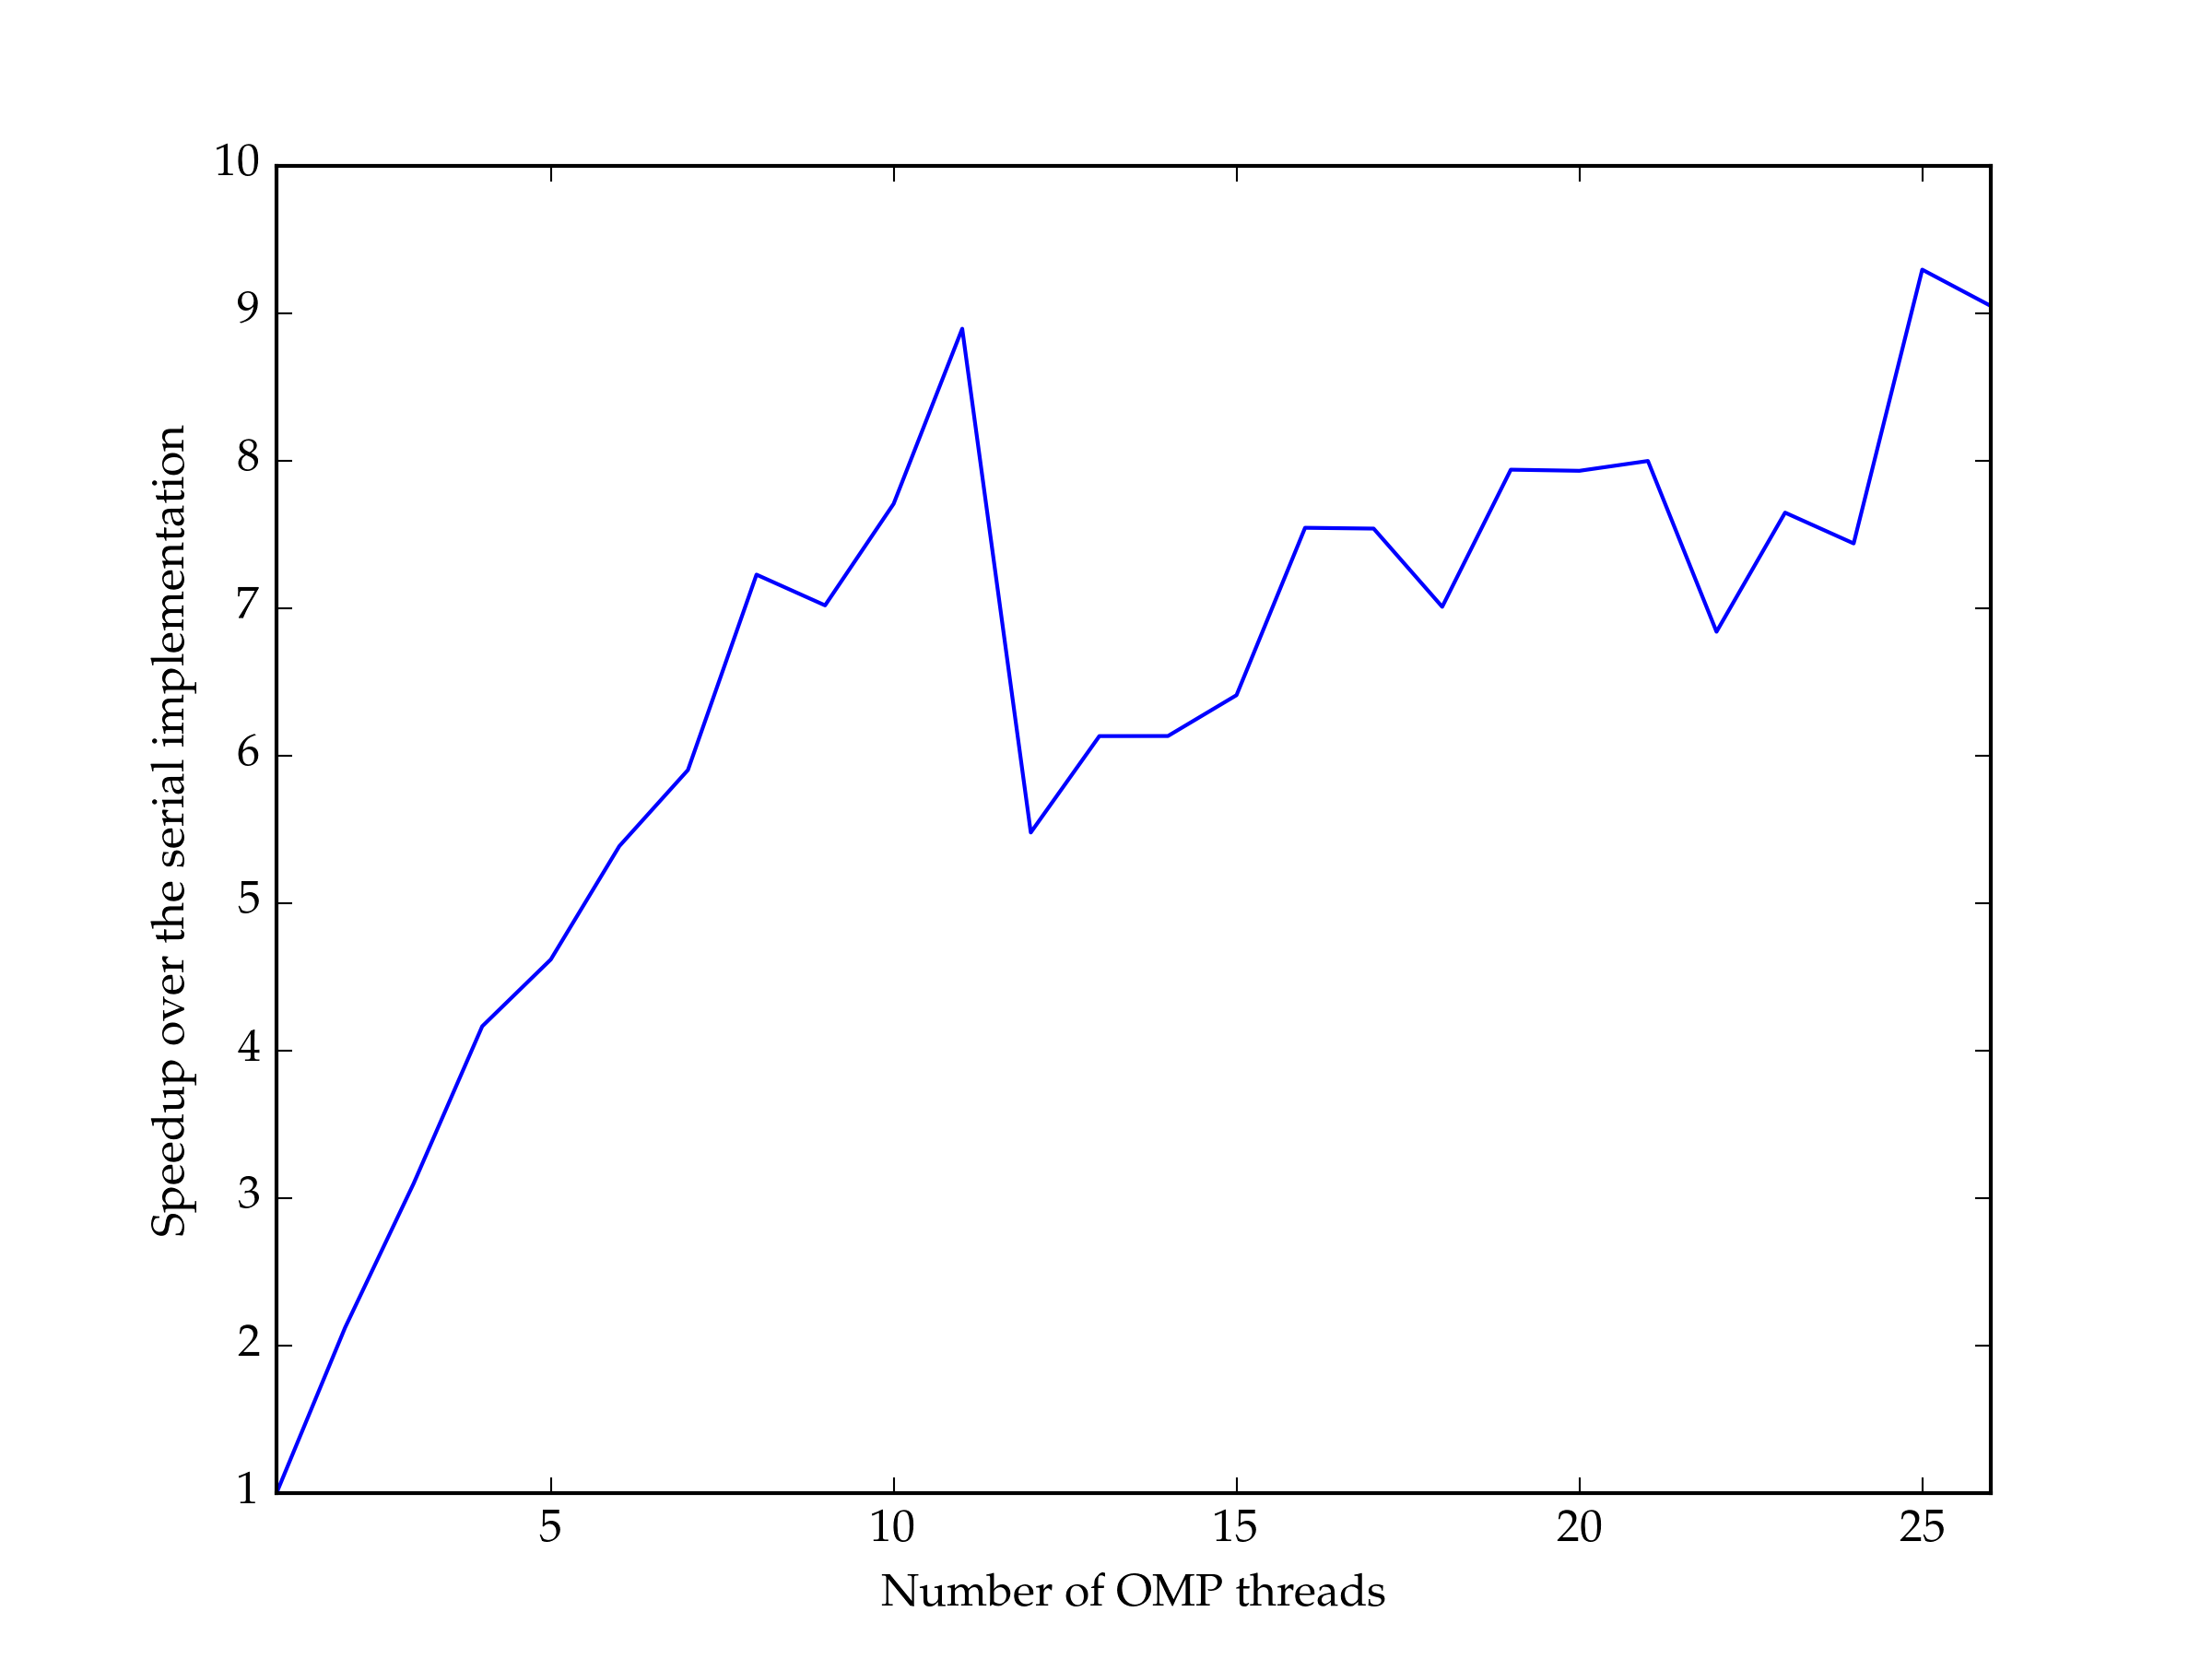
\includegraphics[scale=0.5]{./scaling_studies/strong_scaling_elliot.png}
\caption{Strong scaling study of the tuned parallel solution}
\label{fig:ss_elliot}
\end{figure}

\begin{figure}[H]
\centering
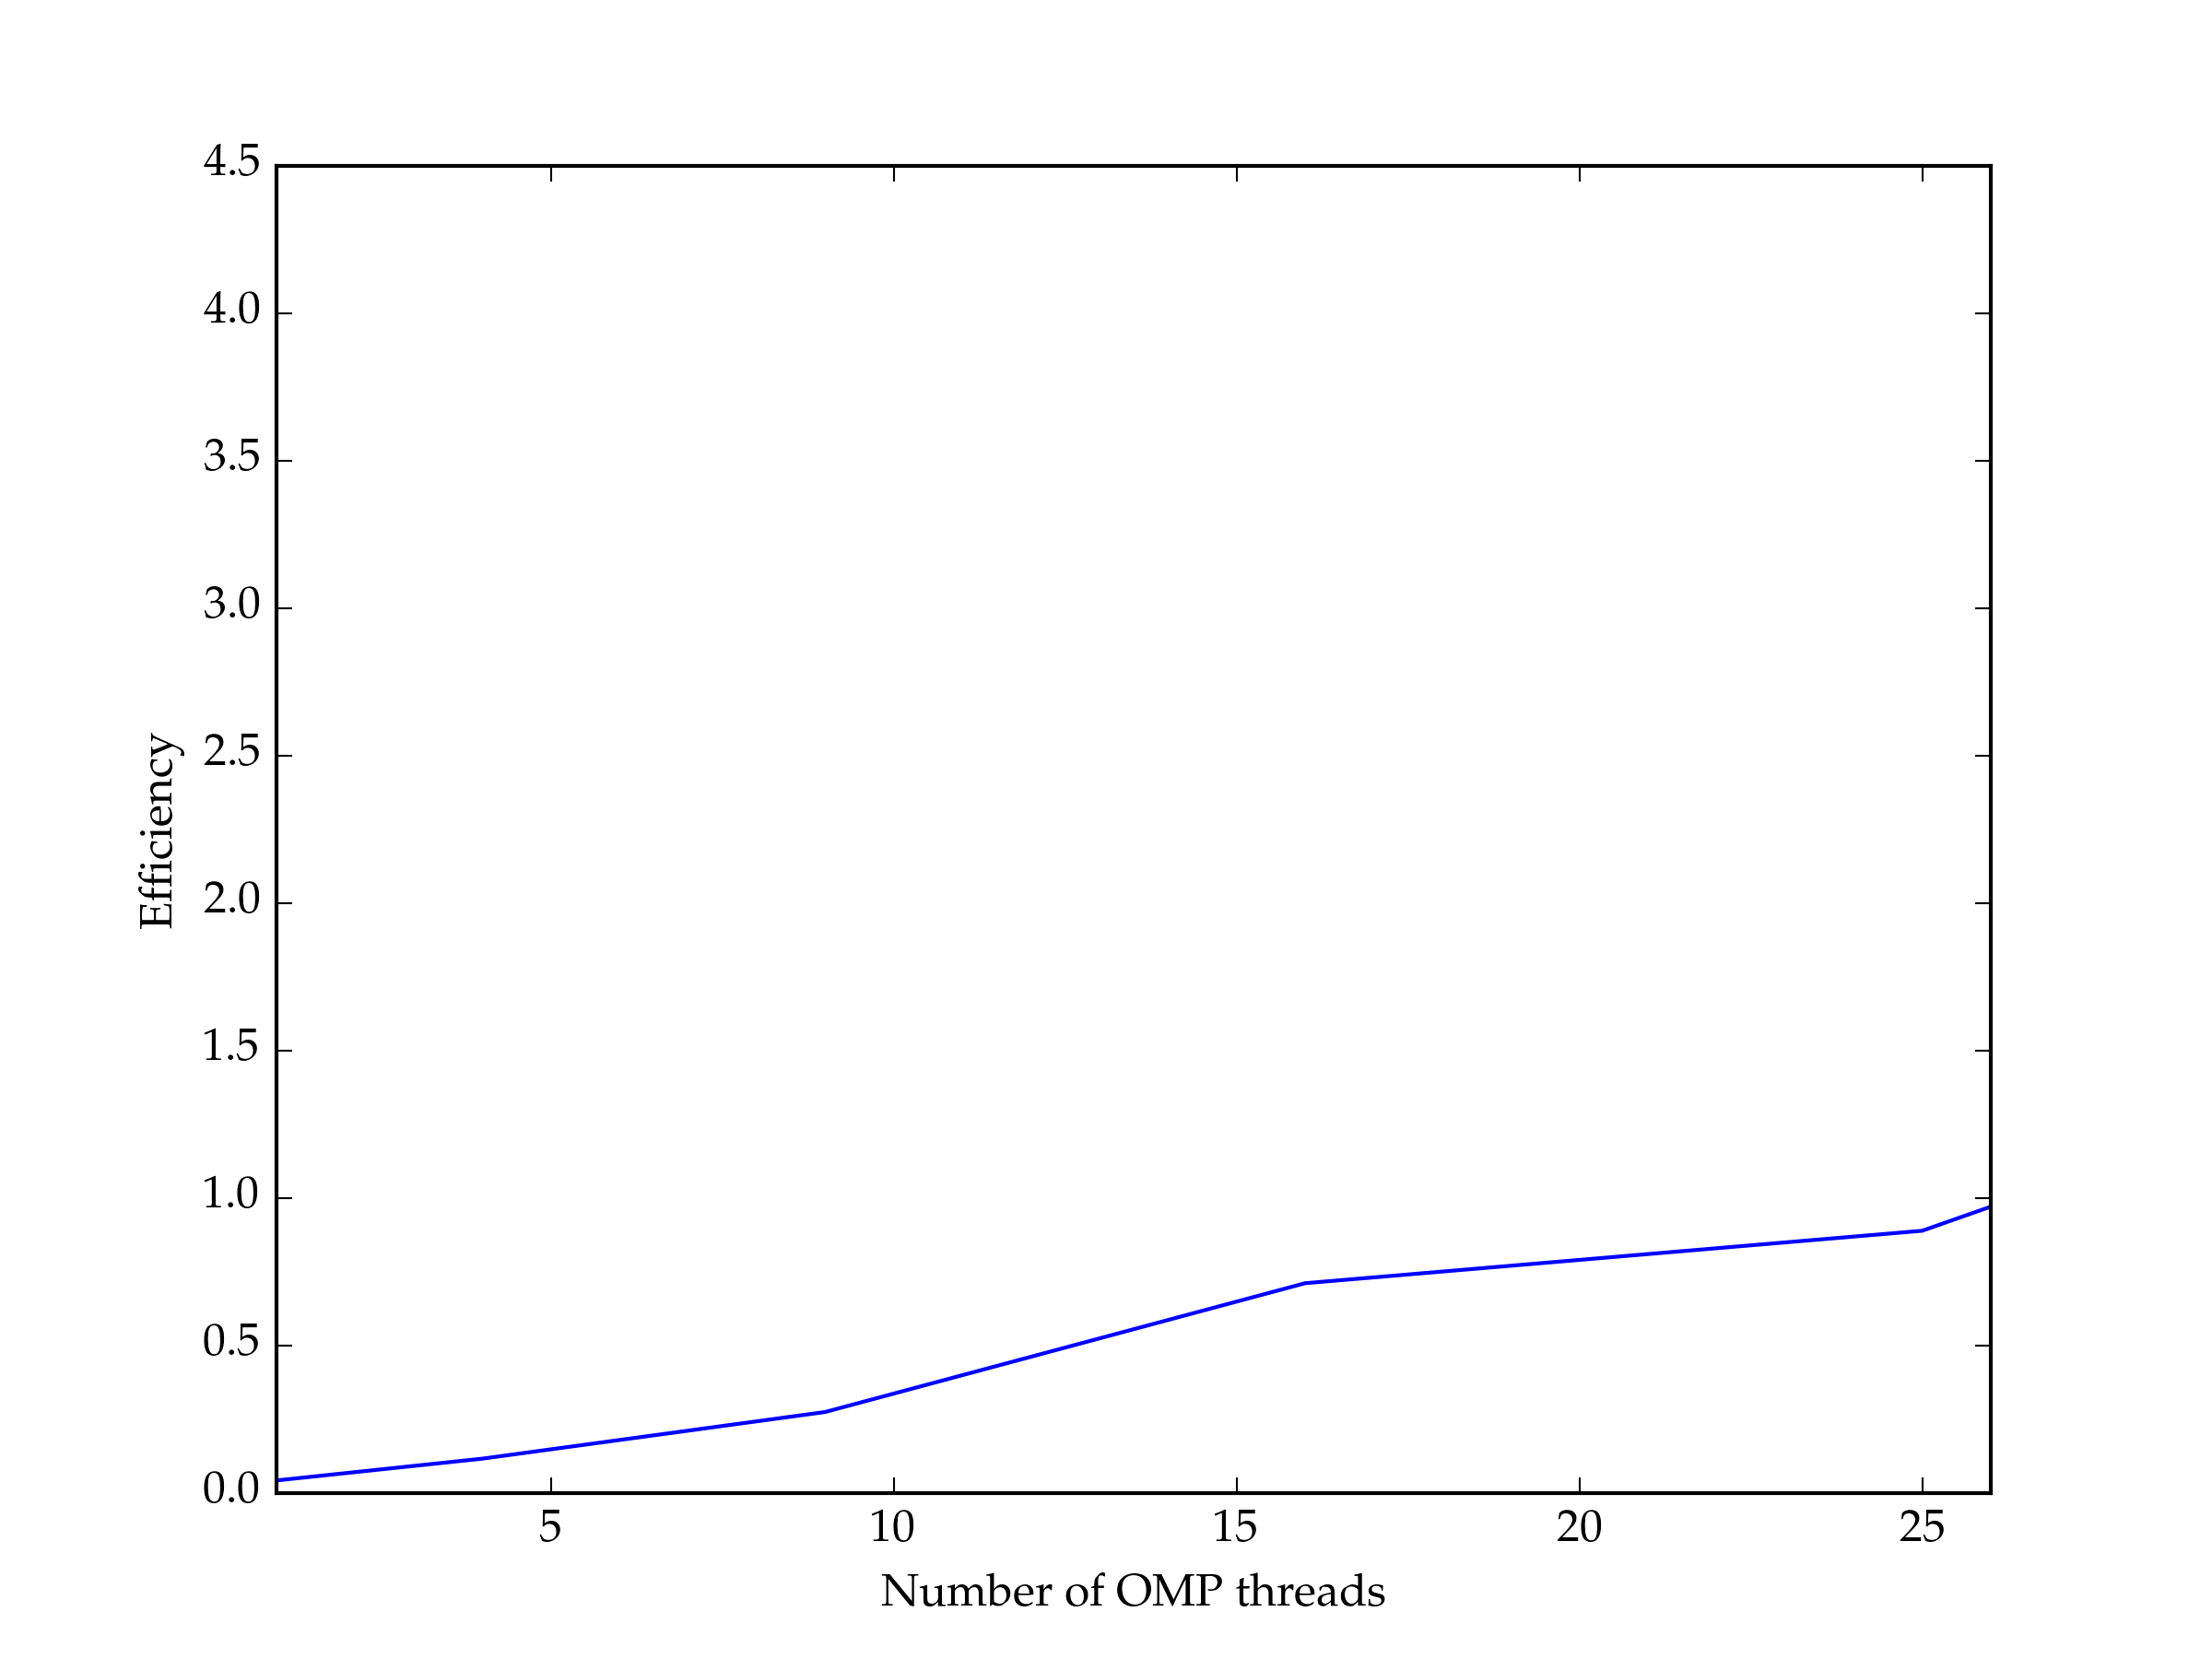
\includegraphics[scale=0.5]{./scaling_studies/weak_scaling_elliot.png}
\caption{Weak scaling study of the tuned parallel solution}
\label{fig:ws_elliot}
\end{figure}

The strong scaling study was performed on a graph with 2048 nodes. The weak scaling varies the number of threads but keeps the problem size per processor be 512 nodes. 

\begin{thebibliography}{9}
\bibitem{writeup}
Bindel, D. \textit{All-Pairs Shortest Paths}. Retrieved November 10, 2015, from \url{https://github.com/sheroze1123/path/blob/master/main.pdf}

\bibitem{cannon}
Hyuk-Jae Lee, James P. Robertson, and Jos� A. B. Fortes. 1997. \textit{Generalized Cannon's algorithm for parallel matrix multiplication}. In Proceedings of the 11th international conference on Supercomputing (ICS '97). ACM, New York, NY, USA, 44-51. DOI=http://dx.doi.org/10.1145/263580.263591

\end{thebibliography}

 
 
\end{document}
